\section{Results}
\label{sec:results}

All the data were preprocessed with Python 3.7.0, while the deep learning and machine learning models were trained and tested using Tensorflow 2.4.0 and PyTorch 2.0.1 modules, respectively. 

The total amount of data from all the horses was 16,500 seconds (or 3,300,000 samples). The estimation accuracy of the trained models with different datasets and their respective optimized hyperparameters are presented in Table \ref{results_fatigue_chap}, where the hyperparameters were labeled with "\#" as their column headers, corresponding to the same number from "\#" column in Table \ref{hyperparameters_fatigue_chap}. Moreover, the estimation results of the best performing models between \gls{imu}+\gls{hr} and \gls{hr} training datasets are compared in a scatter plot (Figure \ref{result_fig_fatigue_chap}). In addition, we showcased the most significant features based on the both-\gls{imu}s dataset in Table \ref{results_features_fatigue_chap}. Moreover, using $\Delta HR$ and the coefficients (b, c) derived from the fitting, the $LA_g$ of each participant was determined independently. The $LA_g$ output of one of the participants is also displayed in Figure \ref{result_lac_fatigue_chap}.

\begin{table}[htbp]
    \centering
        \caption{Best set of hyperparameters and performance metrics of the trained models}

         \resizebox{0.95\linewidth}{!}{% 
    \begin{tabular}{llcccccc}
    \toprule
        \textbf{Model} & \textbf{Input} & \multicolumn{4}{c}{\textbf{Hyperparameters}} & \textbf{RMSE} & \textbf{MAPE} \\ \cline{3-6} 
        ~ & ~ & \textbf{\#1} & \textbf{\#2} & \textbf{\#3} & \textbf{\#4} & \textbf{(mmol/L)} & \textbf{(\%)} \\ \hline
        CNN & IMU+HR & 32, 128 & Constant  & \{7\}, \{2\}  & 128  & 0.11  & 4.89  \\ 
        ~ & Both-IMUs & 32, 128 & Constant  & \{7\}, \{2\}  & 128  & 0.22  & 8.72  \\ 
        ~ & Sacrum IMU & 128, 128 & Constant  & \{5\}, \{3\}  & 128  & 0.25  & 9.60  \\
        ~ & Limb IMU & 64, 64 & Adaptive  & \{7\}, \{2\}  & 128  & 0.32  & 11.79  \\ \hline
        LSTM & IMU+HR & 75 & Adaptive  & -  & -  & 0.14  & 4.51  \\ 
        ~ & Both-IMUs & 75 & Adaptive  & -  & -  & 0.26  & 9.70  \\ 
        ~ & Sacrum IMU & 100 & Constant  & -  & -  & 0.30  & 11.95  \\ 
        ~ & Limb IMU & 50 & Constant  & -  & -  & 0.38  & 13.62  \\ \hline
        Neural networks & HR & - & -  & -  & -  & 0.79  & 28.54  \\ 
        ~ & IMU+HR & (N) & Constant  & 0.0001  & -  & 0.74  & 35.14  \\ 
        ~ & Both-IMUs & (N) & Constant  & 0.001  & -  & 0.80  & 38.11  \\ 
        ~ & Sacrum IMU & (N) & Constant  & 0.001  & -  & 0.86  & 39.73  \\ 
        ~ & Limb IMU & (N) & Constant  & 0.0001  & -  & 0.98  & 46.11  \\ \hline
        Random forest & HR & - & -  & -  & -  & 0.38  & 13.73  \\ 
        ~ & IMU+HR & 10 & $N^2$  & 2  & 50  & 0.24  & 9.85  \\ 
        ~ & Both-IMUs & None & $N^2$  & 2  & 500  & 0.29  & 10.38  \\ 
        ~ & Sacrum IMU & None & $N^2$  & 2  & 200  & 0.33  & 11.65  \\ 
        ~ & Limb IMU & None & $N^2$  & 2  & 100  & 0.39  & 13.79  \\ \hline
        Decision tree & HR & - & -  & -  & -  & 0.40  & 13.78  \\ 
        ~ & IMU+HR & 10 & $N^2$  & 5  & -  & 0.39  & 13.81  \\ 
        ~ & Both-IMUs & 10 & $N^2$  & 10  & -  & 0.46  & 19.73  \\ 
        ~ & Sacrum IMU & None & $N^2$  & 8  & -  & 0.52  & 22.55  \\ 
        ~ & Limb IMU & 10 & $N^2$  & 2  & -  & 0.54  & 21.76  \\ \bottomrule
    \end{tabular}}
    \label{results_fatigue_chap}
\end{table}

\begin{figure}[htb]
\centering
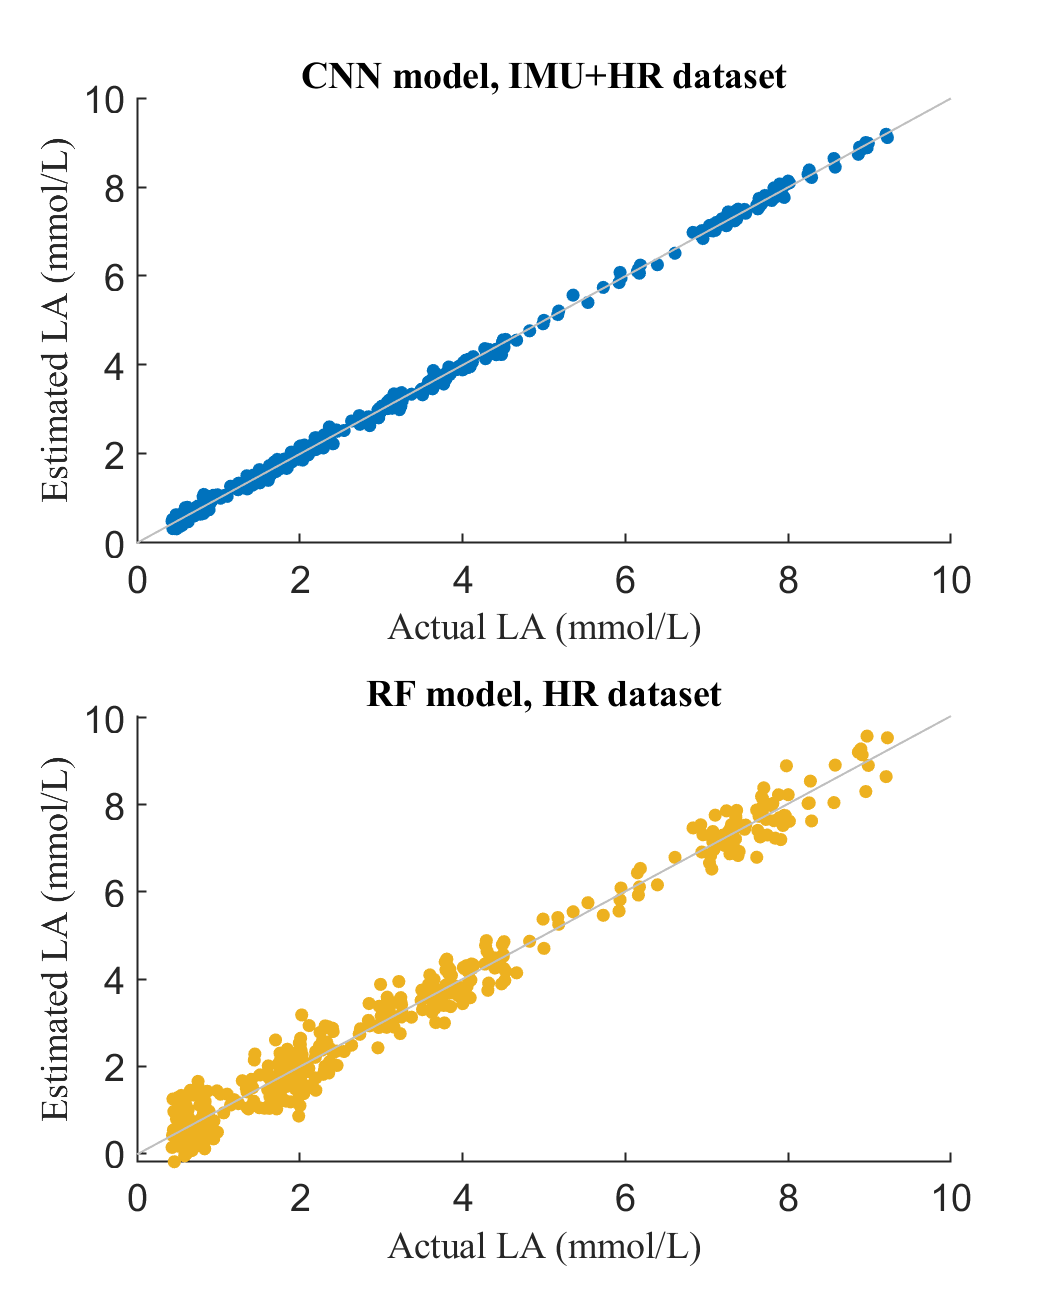
\includegraphics[width=.65\linewidth]{chapters/fatigue/figures/Picture5.png}
\caption{Examples of estimated \gls{lac} over a participant \gls{set} from (above) \gls{cnn} model, \gls{imu}+\gls{hr} training dataset and (below) random forest model, \gls{hr} training dataset.}
\label{result_fig_fatigue_chap}
\end{figure}

\begin{table}[htb]
    \centering
    \caption{The ten highest ranking features from NCA}
     \resizebox{0.95\linewidth}{!}{% 
    \begin{tabular}{lllll}
    \toprule
        \textbf{Rank} & \textbf{Feature description} & \textbf{IMU} & \textbf{Signal/Feature} & \textbf{Axis/Angle} \\ \hline
        1 & Spectral energy & Sacrum & Ang. Velocity & Roll \\ 
        2 & Spectral energy & Limb & Ang. Velocity & Protraction/Retraction  \\ 
        3 & NSEF & Both & Kinematic & Longitudinal  \\ 
        4 & AROM & Limb & Kinematic  & Abduction/Adduction \\ 
        5 & Sum of FFT 1st 3 coefficients  & Sacrum & Ang. Velocity & Yaw  \\ 
        6 & Spectral energy & Sacrum & Acceleration & Vertical  \\ 
        7 & AROM & Limb & Kinematic  & Protraction/Retraction  \\ 
        8 & Stride regularity & Sacrum & Acceleration & Vertical  \\ 
        9 & Standard deviation & Sacrum & Acceleration & Longitudinal  \\ 
        10 & Maximum & Sacrum & Acceleration & Vertical \\ \bottomrule
    \end{tabular}}
    \label{results_features_fatigue_chap}
\end{table}


\begin{figure}[htb]
\centering
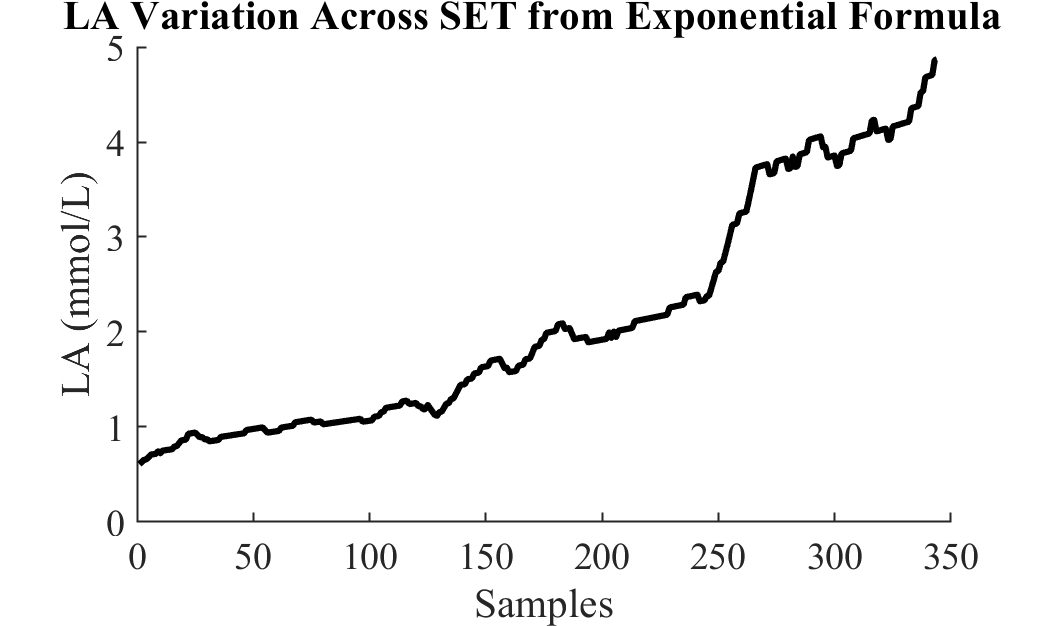
\includegraphics[width=.65\linewidth]{chapters/fatigue/figures/Picture6.png}
\caption{An example of $LA_g$ over a participant \gls{set} calculated using the exponential formula.}
\label{result_lac_fatigue_chap}
\end{figure}

Overall, the deep learning models performed better than the baseline models, where the best and the worst performing models were based on \gls{cnn} and neural networks, respectively. The ranges of performance metrics were 0.11-0.98 \gls{mmol/L} for accuracy and 4.51\% to 46.11\% for relative error. Setting the window size to four seconds resulted in improved performance for all the models. 

 It can be inferred from Table \ref{results_fatigue_chap} that the \gls{cnn} and \gls{lstm} models based on \gls{imu}+\gls{hr} training dataset yielded the best accuracy (0.11 \gls{mmol/L}) and lowest relative error (4.51\%). Between models based on single \gls{imu}, the \gls{cnn} model based on the sacrum \gls{imu} presented higher accuracy and lower relative error (0.25 \gls{mmol/L}, 9.6\%) than the limb \gls{imu} (0.32 \gls{mmol/L}, 11.79\%). Furthermore, the model accuracy increased whenever \gls{hr} was added to the \gls{imu} features (Best: \gls{cnn}, 0.11 \gls{mmol/L}, 4.89\%). In contrast, the accuracy decreased when \gls{hr} was considered as the only input feature (Best: random forest, 0.39 \gls{mmol/L}, 13.73\%).  
 The ten most relevant features for $LA_g$ estimation were selected using \gls{nca} and are presented in Table \ref{results_features_fatigue_chap}. Five and three out of the ten features relied on the sacrum and limb \gls{imu}, whereas two features were independent of the \gls{imu} (i.e. extractable from sacrum or limb \gls{imu}). Moreover, three features were kinematics parameters, while the remaining were signal-based features. 

 The accuracy of the model using the Endurance horses data is presented in Figure \ref{results_fatigue_endur}. The \gls{lac} estimation percentage error columns and error bars presented in the Figure are the average and the standard deviation of all endurance horses that were tested. As indicated in Table \ref{tab:IMU info on horses}, it is important to note that the \gls{hr} of N8 and N15 was not measured, resulting in the absence of results for these horses in the \gls{imu}+\gls{hr} dataset. 

\begin{figure}[htb]
\centering
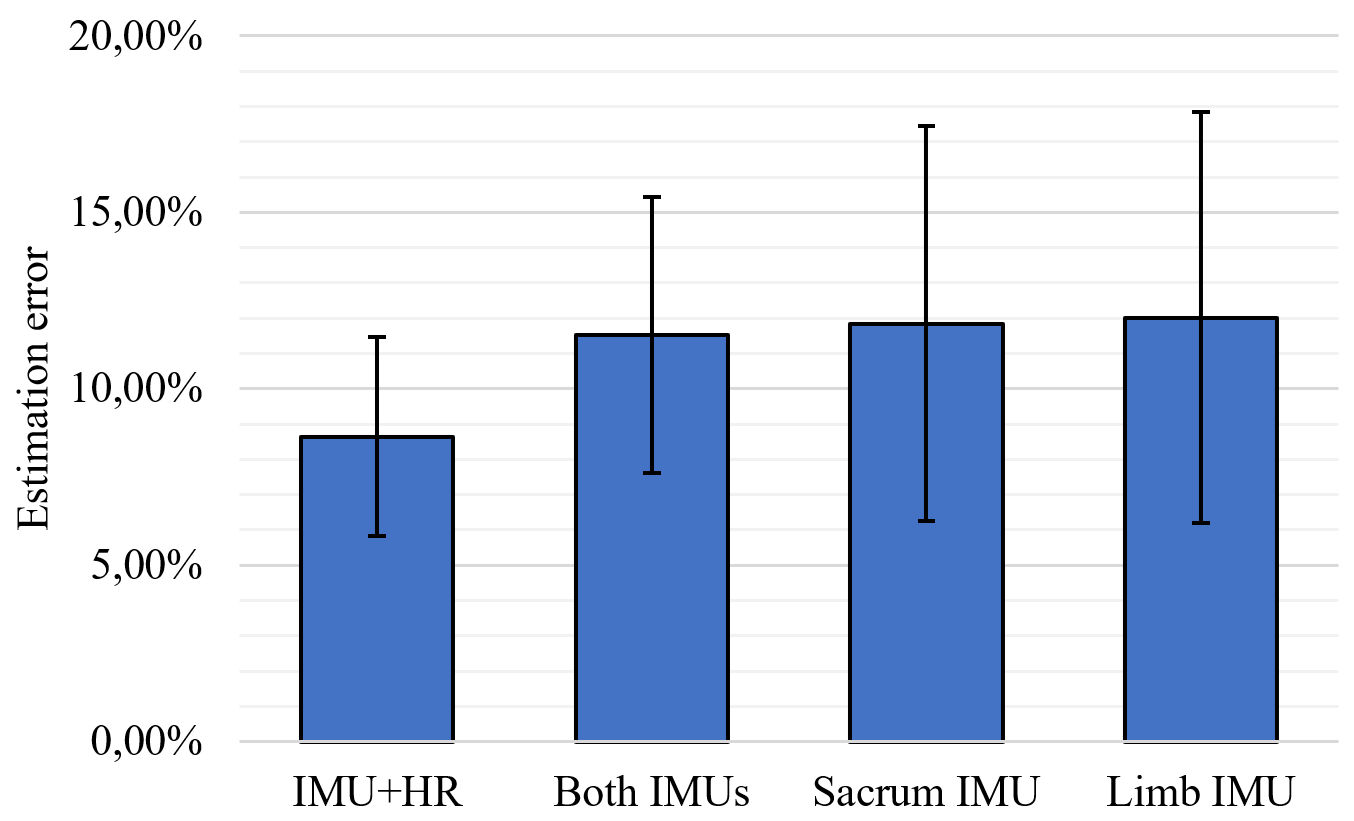
\includegraphics[width=.65\linewidth]{chapters/fatigue/figures/Picture8.png}
\caption{The \gls{lac} estimation percentage errors of the trained \gls{cnn} models on the endurance horses \gls{set} data. The error bars are the standard deviation of the estimation percentage errors.}
\label{results_fatigue_endur}
\end{figure}
 